\documentclass{beamer}
\usetheme{Madrid}
\usepackage{graphicx}
\usepackage{array}
\usepackage{ragged2e}
\usepackage{comment}
\usepackage{amsmath}
\usepackage{tikz}
\usepackage{pgfplots}
\pgfplotsset{compat=1.18}
\usepackage{booktabs}
\usepackage{algorithm}
\usepackage{algpseudocode}
\usepackage{longtable}
\usetikzlibrary{patterns, shapes.geometric, arrows, positioning}

\setbeamertemplate{footline}{}
\setbeamertemplate{navigation symbols}{}

\title[EV Charging Station]{Edge-Driven Semi-Autonomous EV Charging Station Using Quantized Vision Models and Real-Time License Plate Recognition}
\author{
  Izz Al Din Noufel Mukthar \quad MDL22CSBS026\\
  Joel K George \quad MDL22CSBS029\\
  Sarah Ann Pothen \quad MDL22CSBS050\\
  Shahma Fathima \quad MDL22CSBS053
}
\institute{Department of Computer Engineering\\Model Engineering College}
\date{April 2026}

\begin{document}

% FRAME 1
\begin{frame}
    \titlepage
\end{frame}

% FRAME 2
\begin{frame}{Contents (1/3)}
  \tableofcontents[sections={1-4}]
\end{frame}

% FRAME 3
\begin{frame}{Contents (2/3)}
  \tableofcontents[sections={5-9}]
\end{frame}

% FRAME 4
\begin{frame}{Contents (3/3)}
  \tableofcontents[sections={10-14}]
\end{frame}

\section{Introduction}

% FRAME 5
\begin{frame}
    \centering
    \Huge Introduction
\end{frame}

% FRAME 6
\begin{frame}{Global EV Adoption Surge}
\begin{itemize}
    \item Unprecedented growth in Electric Vehicle (EV) adoption worldwide.
    \item Global EV sales surpassed 14 million units in 2023.
    \item Represents a massive year-over-year increase of 35\%.
    \item Cumulative number of EVs on roads crossed 40-million globally.
\end{itemize}
\end{frame}

% FRAME 7
\begin{frame}{Market Projections}
\begin{itemize}
    \item Projections: EVs will be $>60\%$ of new car sales by 2030 in leading markets.
    \item Key markets include China, Europe, and North America.
    \item This rapid expansion places enormous pressure on charging infrastructure.
\end{itemize}
\end{frame}

% FRAME 8
\begin{frame}{Infrastructure Strain}
\begin{itemize}
    \item The infrastructure must scale in capacity to meet demand.
    \item Crucially, it must also scale in usability and seamlessness.
    \item Current systems suffer from complex user-interaction paradigms.
\end{itemize}
\end{frame}

% FRAME 9
\begin{frame}{The Charging Experience Bottleneck}
\begin{itemize}
    \item High-power hardware (Level 2 AC, DC fast chargers) is deploying rapidly.
    \item However, the user experience at public stations remains a major bottleneck.
    \item The transition from petrol stations to EV charging stations introduces significant new friction.
\end{itemize}
\end{frame}

\section{The Indian Context}

% FRAME 10
\begin{frame}
    \centering
    \Huge The Indian Context
\end{frame}

% FRAME 11
\begin{frame}{Accelerated Adoption in India}
\begin{itemize}
    \item India has witnessed a dramatic acceleration in EV adoption.
    \item Propelled by the FAME II scheme (Faster Adoption and Manufacturing of EVs).
    \item EV sales surged from $\sim$5,000 units in 2018 to $>1.5$ million in 2023.
\end{itemize}
\end{frame}

% FRAME 12
\begin{frame}{Infrastructure Goals in India}
\begin{itemize}
    \item Government target: 30\% EV penetration by 2030.
    \item Current network: $\sim$12,000 public charging stations.
    \item Required expansion: An estimated 400,000 stations nationwide.
    \item Streamlining the charging process is essential for this scale.
\end{itemize}
\end{frame}

\section{Friction in Current Systems}

% FRAME 13
\begin{frame}
    \centering
    \Huge Current Friction Points
\end{frame}

% FRAME 14
\begin{frame}{The App-Centric Model}
\begin{itemize}
    \item The prevailing interaction model is entirely smartphone-centric.
    \item Drivers must engage with operator-specific smartphone applications.
    \item Requires downloading, registering, authenticating, and initiating sessions.
\end{itemize}
\end{frame}

% FRAME 15
\begin{frame}{Network Fragmentation}
\begin{itemize}
    \item The network is highly fragmented among competing operators.
    \item Operators like Tata Power, ChargeZone, and Ather Grid use distinct ecosystems.
    \item A driver visiting five networks must maintain five separate apps and wallets.
\end{itemize}
\end{frame}

\section{Motivation}

% FRAME 16
\begin{frame}
    \centering
    \Huge Motivation
\end{frame}

% FRAME 17
\begin{frame}{Motivation: App Fatigue}
\begin{itemize}
    \item Research: 67\% of EV drivers express frustration with multiple apps.
    \item Average public session involves 4--7 discrete digital interaction steps.
    \item Contrasts sharply with a traditional petrol pump "swipe and go" gesture.
\end{itemize}
\end{frame}

% FRAME 18
\begin{frame}{Motivation: Connectivity Dependency}
\begin{itemize}
    \item Cloud authentication inherently depends on stable cellular networks.
    \item Chargers are often in areas with poor cellular coverage:
    \begin{itemize}
        \item Underground parking garages.
        \item Remote highway rest stops.
    \end{itemize}
    \item Connection failures prevent session initiation entirely.
\end{itemize}
\end{frame}

% FRAME 19
\begin{frame}{Motivation: Accessibility Gaps}
\begin{itemize}
    \item App-centric models disproportionately exclude certain demographics.
    \item Elderly users or individuals with limited smartphone proficiency face barriers.
    \item Tourists without local SIM cards cannot access regional networks.
\end{itemize}
\end{frame}

% FRAME 20
\begin{frame}{Motivation: Edge Computing Maturity}
\begin{itemize}
    \item Edge computing brings intelligence directly to the point of service.
    \item Affordable single-board computers (Raspberry Pi 4B) now provide sufficient power.
    \item Quantization enables massive models to run efficiently on resource-constrained devices.
\end{itemize}
\end{frame}

\section{Objectives}

% FRAME 21
\begin{frame}
    \centering
    \Huge Objectives
\end{frame}

% FRAME 22
\begin{frame}{Primary Objectives}
\begin{itemize}
    \item Develop an Automatic License Plate Recognition (ALPR) system for edge deployment.
    \item Quantize a YOLOv11 object detection model from FP32 to INT8 precision.
    \item Achieve $>85\%$ model size reduction with $<2\%$ accuracy degradation.
\end{itemize}
\end{frame}

% FRAME 23
\begin{frame}{Technical Objectives}
\begin{itemize}
    \item Resolve INT8 operator incompatibility on ARM via custom ONNX graph patching.
    \item Implement an asynchronous WebSocket server for real-time frame processing.
    \item Build a native iOS client application for camera streaming with live overlays.
\end{itemize}
\end{frame}

\section{Scope}

% FRAME 24
\begin{frame}
    \centering
    \Huge Scope
\end{frame}

% FRAME 25
\begin{frame}{Scope \& Boundaries}
\begin{itemize}
    \item \textbf{In Scope:} Model fine-tuning, ONNX graph patching, Raspberry Pi edge server, iOS client app, SQLite DB integration.
    \item \textbf{Out of Scope:} Physical charger hardware integration (GPIO), production-grade payment gateways, non-Indian plate formats.
\end{itemize}
\end{frame}

\section{Problem Statement}

% FRAME 26
\begin{frame}
    \centering
    \Huge Problem Statement
\end{frame}

% FRAME 27
\begin{frame}{The Core Issue}
\begin{itemize}
    \item Current stations require multi-step digital workflows via smartphone apps.
    \item Creates significant friction, connectivity dependencies, and accessibility barriers.
    \item Identifying vehicles and processing payments is slow and cumbersome.
\end{itemize}
\end{frame}

% FRAME 28
\begin{frame}{Typical Charging Workflow (Steps 1-4)}
\begin{enumerate}
    \item Driver locates an available charger.
    \item Identifies the specific charging network operator.
    \item Downloads the operator's app (if not installed).
    \item Creates an account and adds a payment method.
\end{enumerate}
\end{frame}

% FRAME 29
\begin{frame}{Typical Charging Workflow (Steps 5-8)}
\begin{enumerate}
    \setcounter{enumi}{4}
    \item Opens app, scans QR code on charger.
    \item Selects charging plan and confirms payment via cloud.
    \item Charging session begins.
    \item Receives notification upon completion.
\end{enumerate}
\end{frame}

% FRAME 30
\begin{frame}{The Research Question}
\begin{block}{Question}
How can we develop a system that automatically identifies registered vehicles upon arrival and authorizes charging sessions without requiring any smartphone interaction, while deploying efficiently on resource-constrained edge hardware?
\end{block}
\end{frame}

\section{Proposed Solution}

% FRAME 31
\begin{frame}
    \centering
    \Huge Proposed Solution
\end{frame}

% FRAME 32
\begin{frame}{Our Edge-Driven Solution}
\begin{itemize}
    \item A semi-autonomous EV charging station powered by edge-based computer vision.
    \item Replaces the 8-step manual workflow with a single autonomous step.
    \item \textbf{The New Workflow:} Vehicle parks $\to$ Camera detects plate $\to$ Edge server authorizes charging.
\end{itemize}
\end{frame}

% FRAME 33
\begin{frame}{Solution Pipeline Overview}
\begin{itemize}
    \item Live camera feed captured by client (iOS/CSI).
    \item Transmitted via low-latency WebSocket to Raspberry Pi.
    \item YOLOv11 INT8 detects license plates.
    \item EasyOCR extracts alphanumeric characters.
    \item Regex validation and SQLite lookup finalize authorization.
\end{itemize}
\end{frame}

% FRAME 34
\begin{frame}{Hardware Deployment}
\begin{itemize}
    \item The entire processing pipeline runs on a \$55 Raspberry Pi 4B.
    \item No cloud server required for the critical authentication window.
    \item Operates securely within the station's Local Area Network.
\end{itemize}
\end{frame}

% FRAME 35
\begin{frame}{Zero-Interaction Experience}
\begin{itemize}
    \item True "Park and Plug" experience.
    \item No smartphones, RFID cards, or QR codes needed.
    \item High degree of privacy as visual data never leaves the edge device.
\end{itemize}
\end{frame}

\section{Key Innovations}

% FRAME 36
\begin{frame}
    \centering
    \Huge Key Innovations
\end{frame}

% FRAME 37
\begin{frame}{Key Innovations Highlighted}
\begin{itemize}
    \item \textbf{Aggressive Quantization:} Reducing YOLOv11 from 200 MB (FP32) to 25 MB (INT8) while maintaining $\sim$93\% accuracy.
    \item \textbf{ONNX Graph Patching:} Programmatically circumventing ARM CPU architecture limitations by shifting signed INT8 tensors to unsigned UINT8 directly within the protobuf graph.
\end{itemize}
\end{frame}

% FRAME 38
\begin{frame}{Comparison with Existing Approaches}
\begin{table}[]
\centering
\renewcommand{\arraystretch}{1.3}
\footnotesize
\begin{tabular}{|l|c|c|c|c|}
\hline
\textbf{Feature} & \textbf{App-Based} & \textbf{RFID} & \textbf{Cloud ALPR} & \textbf{Ours} \\
\hline
Smartphone Reqd. & Yes & No & No & \textbf{No} \\
Cloud Conn.      & Reqd. & Reqd. & Reqd. & \textbf{Not Reqd.} \\
User Steps       & 5--8 & 2--3 & 0 & \textbf{0} \\
Privacy          & Low & Low & Low & \textbf{High} \\
Latency          & 3--10s & 1--2s & 2--5s & \textbf{$<$1s} \\
Hardware Cost    & Low & Medium & High & \textbf{Low} \\
\hline
\end{tabular}
\end{table}
\end{frame}

\section{Literature Survey}

% FRAME 39
\begin{frame}
    \centering
    \Huge Literature Survey
\end{frame}

% FRAME 40
\begin{frame}{Literature Survey (1/4)}
\begin{itemize}
    \item \textbf{Knowledge Distillation:} Acharya et al. (2024) and Cantini et al. (2024) demonstrated transferring complex logic from massive teacher models to smaller student models.
    \item \textit{Relevance:} Validates that aggressive model compression can retain task-critical reasoning, supporting our INT8 quantization strategy.
\end{itemize}
\end{frame}

% FRAME 41
\begin{frame}{Literature Survey (2/4)}
\begin{itemize}
    \item \textbf{Quantization \& Pruning:} Kim (2023) and Lang et al. (2023) provided hardware-aware surveys of PTQ vs. QAT and uniform quantization.
    \item \textit{Relevance:} Dictated our choice of Post-Training Static Quantization (PTQ) to leverage ARM NEON SIMD optimizations without retraining.
\end{itemize}
\end{frame}

% FRAME 42
\begin{frame}{Literature Survey (3/4)}
\begin{itemize}
    \item \textbf{Edge Computing Paradigm:} Shi et al. (2016) and Yi et al. (2025) highlighted latency, bandwidth, and privacy advantages of processing at the edge.
    \item \textit{Relevance:} Forms the architectural foundation of our zero-cloud-dependency authentication pipeline.
\end{itemize}
\end{frame}

% FRAME 43
\begin{frame}{Literature Survey (4/4)}
\begin{itemize}
    \item \textbf{ALPR \& EV Behavior:} Laroca et al. (2021) identified YOLO as optimal for ALPR. Hardman et al. (2018) identified "app fragmentation" as a primary pain point for EV users.
    \item \textit{Relevance:} Directly motivates the project's core user-experience overhaul and algorithm selection.
\end{itemize}
\end{frame}

\section{System Architecture}

% FRAME 44
\begin{frame}
    \centering
    \Huge System Architecture
\end{frame}

% FRAME 45
\begin{frame}{Architecture Flowchart}
\begin{center}
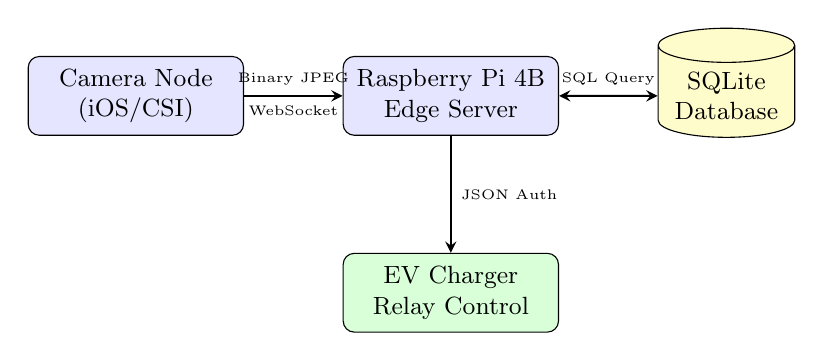
\begin{tikzpicture}[node distance=2.2cm, auto,
    block/.style={rectangle, draw, fill=blue!10, text width=2.5cm, text centered, rounded corners, minimum height=1cm, font=\small},
    db/.style={cylinder, draw, shape border rotate=90, aspect=0.25, fill=yellow!20, text centered, font=\small},
    arrow/.style={thick,->,>=stealth}]
    \node [block] (cam) {Camera Node\\(iOS/CSI)};
    \node [block, right of=cam, node distance=4cm] (pi) {Raspberry Pi 4B\\Edge Server};
    \node [db, right of=pi, node distance=3.5cm, text width=1.5cm, minimum height=1cm] (dbnode) {SQLite\\Database};
    \node [block, below of=pi, node distance=2.5cm, fill=green!15] (charger) {EV Charger\\Relay Control};
    
    \draw [arrow] (cam) -- node[above, font=\tiny]{Binary JPEG} node[below, font=\tiny]{WebSocket} (pi);
    \draw [arrow, <->] (pi) -- node[above, font=\tiny]{SQL Query} (dbnode);
    \draw [arrow] (pi) -- node[right, font=\tiny]{JSON Auth} (charger);
\end{tikzpicture}
\end{center}
\end{frame}

% FRAME 46
\begin{frame}{Use Case Diagram (1/2)}
\begin{center}
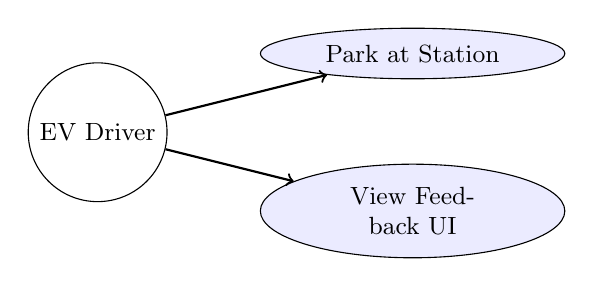
\begin{tikzpicture}[
    actor/.style={circle, draw, minimum size=0.6cm, font=\small},
    usecase/.style={ellipse, draw, fill=blue!8, text width=2.5cm, text centered, minimum height=0.6cm, font=\small},
    arrow/.style={->, thick}
]
\node[actor] (driver) at (0,0) {EV Driver};
\node[usecase] (park) at (4, 1) {Park at Station};
\node[usecase] (view) at (4, -1) {View Feedback UI};
\draw[arrow] (driver) -- (park);
\draw[arrow] (driver) -- (view);
\end{tikzpicture}
\end{center}
\end{frame}

% FRAME 47
\begin{frame}{Use Case Diagram (2/2)}
\begin{center}
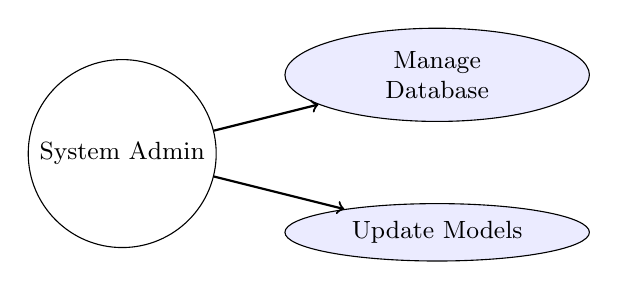
\begin{tikzpicture}[
    actor/.style={circle, draw, minimum size=0.6cm, font=\small},
    usecase/.style={ellipse, draw, fill=blue!8, text width=2.5cm, text centered, minimum height=0.6cm, font=\small},
    arrow/.style={->, thick}
]
\node[actor] (admin) at (0,0) {System Admin};
\node[usecase] (manage) at (4, 1) {Manage Database};
\node[usecase] (update) at (4, -1) {Update Models};
\draw[arrow] (admin) -- (manage);
\draw[arrow] (admin) -- (update);
\end{tikzpicture}
\end{center}
\end{frame}

% FRAME 48
\begin{frame}{Level 0 DFD (Context Diagram) (1/2)}
\begin{itemize}
    \item System establishes boundary limits.
    \item Inputs: JPEG frames from the camera.
    \item Processing: ALPR and authorization logic.
\end{itemize}
\end{frame}

% FRAME 49
\begin{frame}{Level 0 DFD (Context Diagram) (2/2)}
\begin{center}
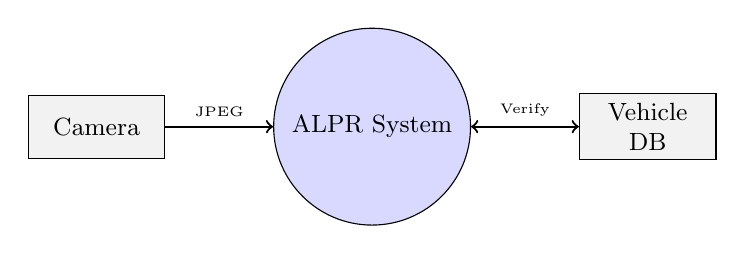
\begin{tikzpicture}[
    entity/.style={rectangle, draw, fill=gray!10, text width=1.5cm, text centered, minimum height=0.8cm, font=\small},
    process/.style={circle, draw, fill=blue!15, minimum size=2.5cm, text centered, font=\small},
    arrow/.style={->, thick}
]
\node[entity] (camera) at (-3.5, 0) {Camera};
\node[process] (system) at (0, 0) {ALPR System};
\node[entity] (db) at (3.5, 0) {Vehicle DB};
\draw[arrow] (camera) -- node[above, font=\tiny]{JPEG} (system);
\draw[arrow, <->] (system) -- node[above, font=\tiny]{Verify} (db);
\end{tikzpicture}
\end{center}
\end{frame}

% FRAME 50
\begin{frame}{Level 1 DFD (Internal Data Flow) (1/2)}
\begin{itemize}
    \item Breaks the system into distinct sequential operations.
    \item Operations: Decode $\to$ Detect $\to$ OCR $\to$ Validate $\to$ Query.
\end{itemize}
\end{frame}

% FRAME 51
\begin{frame}{Level 1 DFD (Internal Data Flow) (2/2)}
\begin{center}
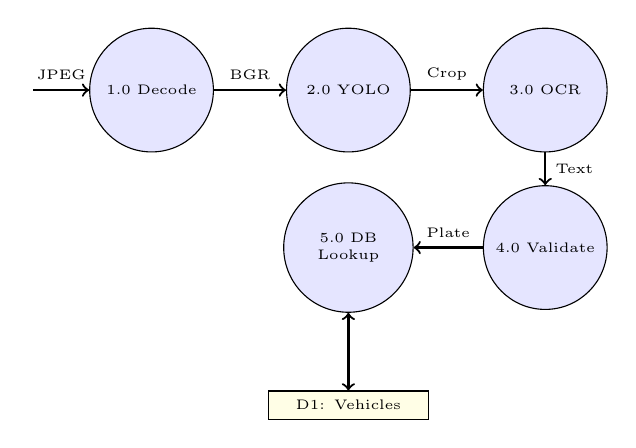
\begin{tikzpicture}[
    process/.style={circle, draw, fill=blue!10, minimum size=1.5cm, text centered, font=\tiny, text width=1.3cm},
    store/.style={rectangle, draw, fill=yellow!10, text width=1.8cm, text centered, font=\tiny},
    arrow/.style={->, thick, font=\tiny}
]
\node[process] (decode) at (0, 0) {1.0 Decode};
\node[process] (yolo) at (2.5, 0) {2.0 YOLO};
\node[process] (ocr) at (5, 0) {3.0 OCR};
\node[process] (validate) at (5, -2) {4.0 Validate};
\node[process] (lookup) at (2.5, -2) {5.0 DB Lookup};
\node[store] (db) at (2.5, -4) {D1: Vehicles};

\draw[arrow] (-1.5, 0) -- node[above]{JPEG} (decode);
\draw[arrow] (decode) -- node[above]{BGR} (yolo);
\draw[arrow] (yolo) -- node[above]{Crop} (ocr);
\draw[arrow] (ocr) -- node[right]{Text} (validate);
\draw[arrow] (validate) -- node[above]{Plate} (lookup);
\draw[arrow, <->] (lookup) -- (db);
\end{tikzpicture}
\end{center}
\end{frame}

% FRAME 52
\begin{frame}{Database ER Diagram}
\begin{center}
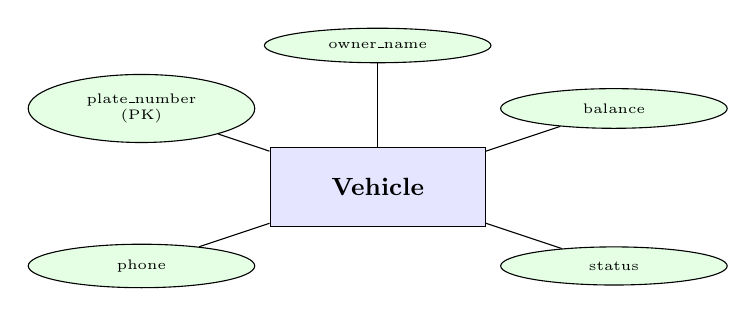
\begin{tikzpicture}[
    entity/.style={rectangle, draw, fill=blue!10, text width=2.5cm, text centered, minimum height=1cm, font=\small},
    attr/.style={ellipse, draw, fill=green!10, text width=1.8cm, text centered, font=\tiny}
]
\node[entity] (vehicle) at (0, 0) {\textbf{Vehicle}};
\node[attr] (plate) at (-3, 1) {plate\_number (PK)};
\node[attr] (owner) at (0, 1.8) {owner\_name};
\node[attr] (balance) at (3, 1) {balance};
\node[attr] (phone) at (-3, -1) {phone};
\node[attr] (status) at (3, -1) {status};
\draw (vehicle) -- (plate);
\draw (vehicle) -- (owner);
\draw (vehicle) -- (balance);
\draw (vehicle) -- (phone);
\draw (vehicle) -- (status);
\end{tikzpicture}
\end{center}
\end{frame}

\section{Modules}

% FRAME 53
\begin{frame}
    \centering
    \Huge Modules \& Processing
\end{frame}

% FRAME 54
\begin{frame}{Module 1: Camera Streaming (iOS)}
\begin{itemize}
    \item Uses AVFoundation \texttt{AVCaptureSession} at \texttt{.vga640x480}.
    \item Flattens raw buffer to \texttt{CIImage} and compresses to JPEG (quality 0.6).
    \item Transmits binary data to the Pi.
    \item Uses SwiftUI \& \texttt{Combine} to dynamically render green bounding boxes and OCR text on screen.
\end{itemize}
\end{frame}

% FRAME 55
\begin{frame}{Module 2: Edge Inference Server}
\begin{itemize}
    \item Decodes frames via OpenCV (\texttt{cv2.imdecode}) in a thread pool.
    \item Prepares frames for YOLO (resize to $640 \times 640$, normalize, NCHW).
    \item Executes INT8 model using \texttt{ONNX Runtime} (aarch64).
    \item Employs Non-Maximum Suppression (NMS) to eliminate duplicate boxes.
\end{itemize}
\end{frame}

% FRAME 56
\begin{frame}{Module 3 \& 4: OCR, Validate, DB}
\begin{itemize}
    \item \textbf{OCR:} EasyOCR (CRNN) processes cropped plate bounding boxes.
    \item \textbf{Validate:} Cleans whitespace and tests against strict Regex pattern: \texttt{\^{}[A-Z]\{2\}[0-9]\{2\}[A-Z]\{1,2\}[0-9]\{4\}\$}
    \item \textbf{Database:} SQLite \texttt{SELECT owner, balance FROM vehicles WHERE plate = ? AND status = 'active'}
\end{itemize}
\end{frame}

% FRAME 57
\begin{frame}{Detection Pipeline Flowchart}
\begin{center}
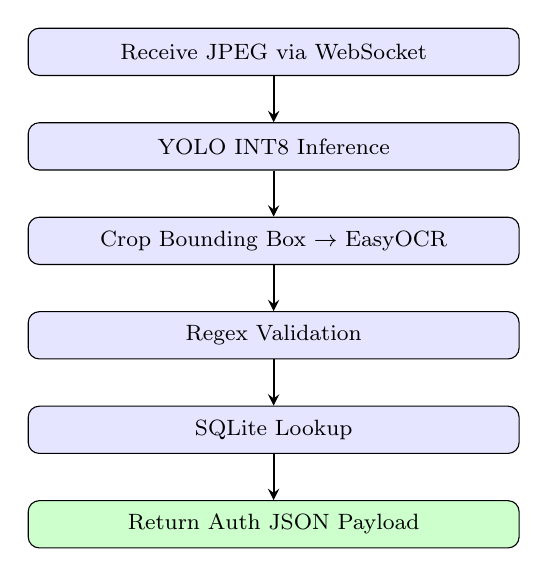
\begin{tikzpicture}[node distance=1.5cm, auto,
    block/.style={rectangle, draw, fill=blue!10, text width=6cm, text centered, rounded corners, minimum height=0.6cm, font=\footnotesize},
    arrow/.style={thick,->,>=stealth}]
    \node [block] (rcv) {Receive JPEG via WebSocket};
    \node [block, below of=rcv, node distance=1.2cm] (yolo) {YOLO INT8 Inference};
    \node [block, below of=yolo, node distance=1.2cm] (crop) {Crop Bounding Box $\to$ EasyOCR};
    \node [block, below of=crop, node distance=1.2cm] (val) {Regex Validation};
    \node [block, below of=val, node distance=1.2cm] (db) {SQLite Lookup};
    \node [block, below of=db, node distance=1.2cm, fill=green!20] (auth) {Return Auth JSON Payload};
    \draw [arrow] (rcv) -- (yolo);
    \draw [arrow] (yolo) -- (crop);
    \draw [arrow] (crop) -- (val);
    \draw [arrow] (val) -- (db);
    \draw [arrow] (db) -- (auth);
\end{tikzpicture}
\end{center}
\end{frame}

% FRAME 58
\begin{frame}{WebSocket Concurrency Model}
\begin{center}
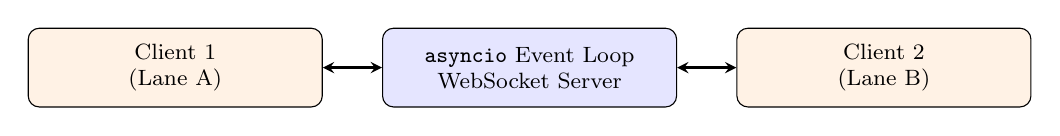
\begin{tikzpicture}[node distance=1.5cm, auto,
    block/.style={rectangle, draw, fill=orange!10, text width=3.5cm, text centered, rounded corners, minimum height=1cm, font=\footnotesize},
    arrow/.style={thick,<->,>=stealth}]
    \node [block] (client1) {Client 1\\(Lane A)};
    \node [block, right of=client1, node distance=4.5cm, fill=blue!10] (server) {\texttt{asyncio} Event Loop\\WebSocket Server};
    \node [block, right of=server, node distance=4.5cm] (client2) {Client 2\\(Lane B)};
    
    \draw [arrow] (client1) -- (server);
    \draw [arrow] (client2) -- (server);
\end{tikzpicture}
\end{center}
\vspace{0.3cm}
\begin{itemize}
    \item \texttt{asyncio} prevents blocking while waiting for network I/O.
    \item CPU-heavy CV tasks are pushed to \texttt{run\_in\_executor} thread pools.
\end{itemize}
\end{frame}

\section{Theoretical Background}

% FRAME 59
\begin{frame}
    \centering
    \Huge YOLO Object Detection
\end{frame}

% FRAME 60
\begin{frame}{YOLO Paradigm}
\begin{itemize}
    \item "You Only Look Once" changed computer vision from classification to regression.
    \item Predicts bounding box coordinates and probabilities in one forward pass.
    \item Extremely fast compared to Region Proposal Networks (e.g., Faster R-CNN).
    \item Implicitly captures global context, reducing false positives in background.
\end{itemize}
\end{frame}

% FRAME 61
\begin{frame}{YOLO Grid Prediction}
\begin{itemize}
    \item Divides image into an $S \times S$ grid.
    \item Cell responsible if object center falls within it.
    \item Each cell predicts $B$ bounding boxes ($x,y,w,h$) + Confidence.
    \item $Validation Score = Pr(\text{Object}) \times \text{IoU}_{pred}^{truth}$
\end{itemize}
\end{frame}

% FRAME 62
\begin{frame}{YOLO Loss Function (1/2)}
Multi-part loss balancing localization and classification:
\begin{equation}
    \mathcal{L} = \mathcal{L}_{coord} + \mathcal{L}_{confidence} + \mathcal{L}_{classification}
\end{equation}
\end{frame}

% FRAME 63
\begin{frame}{YOLO Loss Function (2/2)}
\begin{equation}
\begin{aligned}
    \mathcal{L} = \;&\lambda_{coord} \sum_{i=0}^{S^2} \sum_{j=0}^{B} \mathbb{1}_{ij}^{obj} \left[ (x_i - \hat{x}_i)^2 + (y_i - \hat{y}_i)^2 \right] \\
    &+ \lambda_{coord} \sum_{i=0}^{S^2} \sum_{j=0}^{B} \mathbb{1}_{ij}^{obj} \left[ (\sqrt{w_i} - \sqrt{\hat{w}_i})^2 \dots \right] \\
    &+ \sum_{i=0}^{S^2} \sum_{j=0}^{B} \mathbb{1}_{ij}^{obj} (C_i - \hat{C}_i)^2 + \dots
\end{aligned}
\end{equation}
\end{frame}

% FRAME 64
\begin{frame}
    \centering
    \Huge Quantization Theory
\end{frame}

% FRAME 65
\begin{frame}{Motivation for Quantization}
\begin{itemize}
    \item FP32 models (200MB) exceed edge cache sizes and memory bandwidth limits.
    \item Mapping floating-point weights to 8-bit integers (INT8) shrinks size by $4\times$.
    \item Replaces costly FP MAC operations with integer arithmetic.
\end{itemize}
\end{frame}

% FRAME 66
\begin{frame}{Affine Quantization Math (1/2)}
Maps real values ($x$) to integers ($x_q$) via Scale ($S$) and Zero-Point ($Z$):
\begin{equation}
    x \approx S \times (x_q - Z)
\end{equation}
Forward mapping is clamped:
\begin{equation}
    x_q = \text{clamp}\left( \text{round}\left( \frac{x}{S} \right) + Z, Q_{min}, Q_{max} \right)
\end{equation}
\end{frame}

% FRAME 67
\begin{frame}{Affine Quantization Math (2/2)}
Matrix multiplication ($y = w \cdot x + b$) becomes purely integer:
\begin{equation}
    y_q = \frac{S_w S_x}{S_y} \sum_{i} (w_{q,i} - Z_w)(x_{q,i} - Z_x) + \frac{b}{S_y} + Z_y
\end{equation}
(The multiplier $\frac{S_w S_x}{S_y}$ is pre-computed as a bit-shift offset).
\end{frame}

% FRAME 68
\begin{frame}{Quantization Pipeline Steps}
\begin{enumerate}
    \item \textbf{Export:} PyTorch $\to$ ONNX FP32.
    \item \textbf{Calibration:} Pass 100 representative plates to determine activation min/max.
    \item \textbf{Static Quantization:} Produce INT8 ONNX graph.
    \item \textbf{Patching:} Fix ARM operator incompatibilities.
\end{enumerate}
\end{frame}

\section{Implementation Algorithms}

% FRAME 69
\begin{frame}{Algorithm: Edge Server Handler}
\begin{algorithm}[H]
\caption{WebSocket Connection Handler}
\begin{algorithmic}[1]
\State $image \gets \text{cv2.imdecode}(binary\_frame)$
\State $boxes \gets \text{YOLO.run}(image)$
\For{each $box$ in $boxes$}
    \If{$\text{IoU}(box, prev) > 0.45$} \text{ // NMS}
        \State \textbf{continue}
    \EndIf
    \State $crop \gets \text{image}[y_1:y_2, x_1:x_2]$
    \State $text \gets \text{EasyOCR.readtext}(crop)$
    \State \Call{ValidateAndVerify}{$text$}
\EndFor
\end{algorithmic}
\end{algorithm}
\end{frame}

% FRAME 70
\begin{frame}{Algorithm: Database Verification}
\begin{algorithm}[H]
\caption{Validate and Verify License Plate}
\begin{algorithmic}[1]
\Function{ValidateAndVerify}{$text$}
    \State $clean \gets \text{Uppercase and Remove Spaces}(text)$
    \If{$\text{RegexMatch}(clean, \text{"\^[A-Z]\{2\}[0-9]\{2\}..."})$}
        \State $db \gets \text{SQLiteConnection()}$
        \State $record \gets db.\text{execute("SELECT owner FROM vehicles WHERE plate = ?", } clean)$
        \If{$record \neq \text{Null}$}
            \State \Return \text{JSON Auth Payload}
        \EndIf
    \EndIf
    \State \Return \text{Null}
\EndFunction
\end{algorithmic}
\end{algorithm}
\end{frame}

% FRAME 71
\begin{frame}{Algorithm: ONNX Graph Patching}
\begin{algorithm}[H]
\caption{Fix ConvInteger INT8 for ARM CPUs}
\begin{algorithmic}[1]
\For{each $node$ in $ONNX\_Graph$}
    \If{$node.type == \text{"ConvInteger"}$}
        \State $weights \gets node.inputs[1]$
        \If{$weights.dataType == \text{INT8}$}
            \State $uint8\_weights \gets (weights + 128).cast(\text{UINT8})$
            \State $node.replace(weights, uint8\_weights)$
        \EndIf
    \EndIf
\EndFor
\end{algorithmic}
\end{algorithm}
\end{frame}

\section{Testing \& Results}

% FRAME 72
\begin{frame}
    \centering
    \Huge Testing \& Results
\end{frame}

% FRAME 73
\begin{frame}{Performance Benchmarks}
\begin{table}[]
\centering
\renewcommand{\arraystretch}{1.2}
\footnotesize
\begin{tabular}{lcc}
\toprule
\textbf{Metric} & \textbf{FP32 Model} & \textbf{INT8 Model} \\
\midrule
Model Size (MB) & 200 & 25 \\
Avg. Inference (ms) & 1842 & 487 \\
Speedup Factor & 1.0$\times$ & 3.78$\times$ \\
mAP@0.5 & 0.942 & 0.931 \\
\bottomrule
\end{tabular}
\end{table}
\end{frame}

% FRAME 74
\begin{frame}{Graph: Inference Latency}
\begin{center}
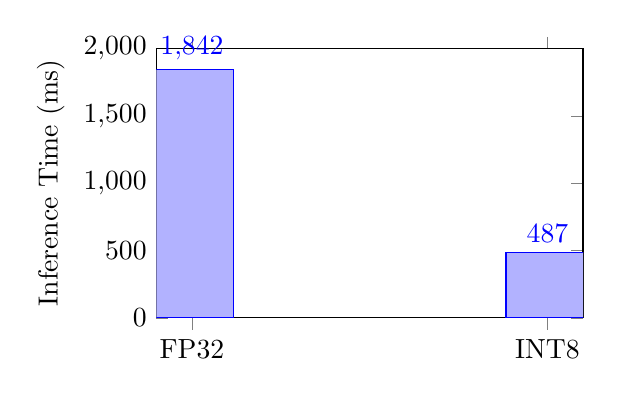
\begin{tikzpicture}
\begin{axis}[
    ybar, bar width=30pt,
    ylabel={Inference Time (ms)},
    symbolic x coords={FP32, INT8},
    xtick=data,
    ymin=0, ymax=2000,
    nodes near coords,
    width=7cm, height=5cm,
    fill=red!40
]
\addplot coordinates {(FP32, 1842) (INT8, 487)};
\end{axis}
\end{tikzpicture}
\end{center}
\end{frame}

% FRAME 75
\begin{frame}{Graph: Peak RAM Usage}
\begin{center}
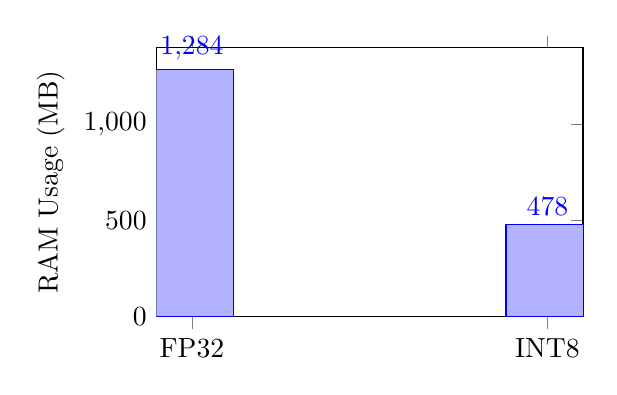
\begin{tikzpicture}
\begin{axis}[
    ybar, bar width=30pt,
    ylabel={RAM Usage (MB)},
    symbolic x coords={FP32, INT8},
    xtick=data,
    ymin=0, ymax=1400,
    nodes near coords,
    width=7cm, height=5cm,
    fill=blue!40
]
\addplot coordinates {(FP32, 1284) (INT8, 478)};
\end{axis}
\end{tikzpicture}
\end{center}
\end{frame}

% FRAME 76
\begin{frame}{Graph: End-to-End Latency Breakdown}
\begin{center}
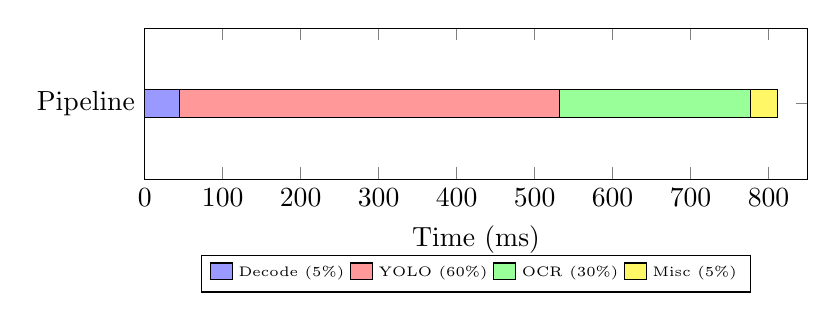
\begin{tikzpicture}
\begin{axis}[
    xbar stacked,
    symbolic y coords={Pipeline},
    ytick=data,
    xlabel={Time (ms)},
    xmin=0, xmax=850,
    height=3.5cm, width=10cm,
    legend style={at={(0.5,-0.5)}, anchor=north, legend columns=4, font=\tiny}
]
\addplot[fill=blue!40] coordinates {(45,Pipeline)};  \addlegendentry{Decode (5\%)}
\addplot[fill=red!40] coordinates {(487,Pipeline)}; \addlegendentry{YOLO (60\%)}
\addplot[fill=green!40] coordinates {(245,Pipeline)}; \addlegendentry{OCR (30\%)}
\addplot[fill=yellow!60] coordinates {(34,Pipeline)}; \addlegendentry{Misc (5\%)}
\end{axis}
\end{tikzpicture}
\end{center}
\end{frame}

% FRAME 77
\begin{frame}{OCR Accuracy Degradation}
\begin{table}[]
\centering
\renewcommand{\arraystretch}{1.2}
\footnotesize
\begin{tabular}{|l|c|c|}
\hline
\textbf{Condition} & \textbf{Character Acc.} & \textbf{Plate Acc.} \\
\hline
Good Lighting & 98.2\% & 94.5\% \\
Low Light & 89.7\% & 78.4\% \\
Distance $>$4m & 85.4\% & 71.8\% \\
\hline
\end{tabular}
\end{table}
\end{frame}

\section{Future Scope \& Conclusion}

% FRAME 78
\begin{frame}
    \centering
    \Huge Future Scope
\end{frame}

% FRAME 79
\begin{frame}{Future Enhancements}
\begin{itemize}
    \item \textbf{GPIO Relay Integration:} Actually trigger physical high-voltage contactors.
    \item \textbf{Cloud Sync:} SQLite to Firebase migration for cross-station roaming.
    \item \textbf{Lighter OCR:} Swap EasyOCR for PaddleOCR-Lite to shave off 100ms.
    \item \textbf{OCPP Integration:} Interface with standard charging protocols.
\end{itemize}
\end{frame}

% FRAME 80
\begin{frame}{Conclusion}
\begin{itemize}
    \item Edge computer vision successfully transforms the EV charging workflow.
    \item Quantization unlocks deep learning on \$55 hardware.
    \item Sub-second latency delivers true "Park and Plug" autonomy.
\end{itemize}
\vspace{0.5cm}
\begin{center}
    \Large \textbf{Thank You!}
\end{center}
\end{frame}

\end{document}
